\chapter{Results \& Analysis}
\section{Analysis \& Discussion}
\subsection{Comparative Analysis}
In order to properly evaluate the performance of our model, we needed a
baseline model to compare against. We chose the original pretrained XFeat
models~\cite{xfeat_github} as they are we try to optimize for our target use
case. The evaluation test yielded the following results:
\begin{figure}[H]
    \centering
    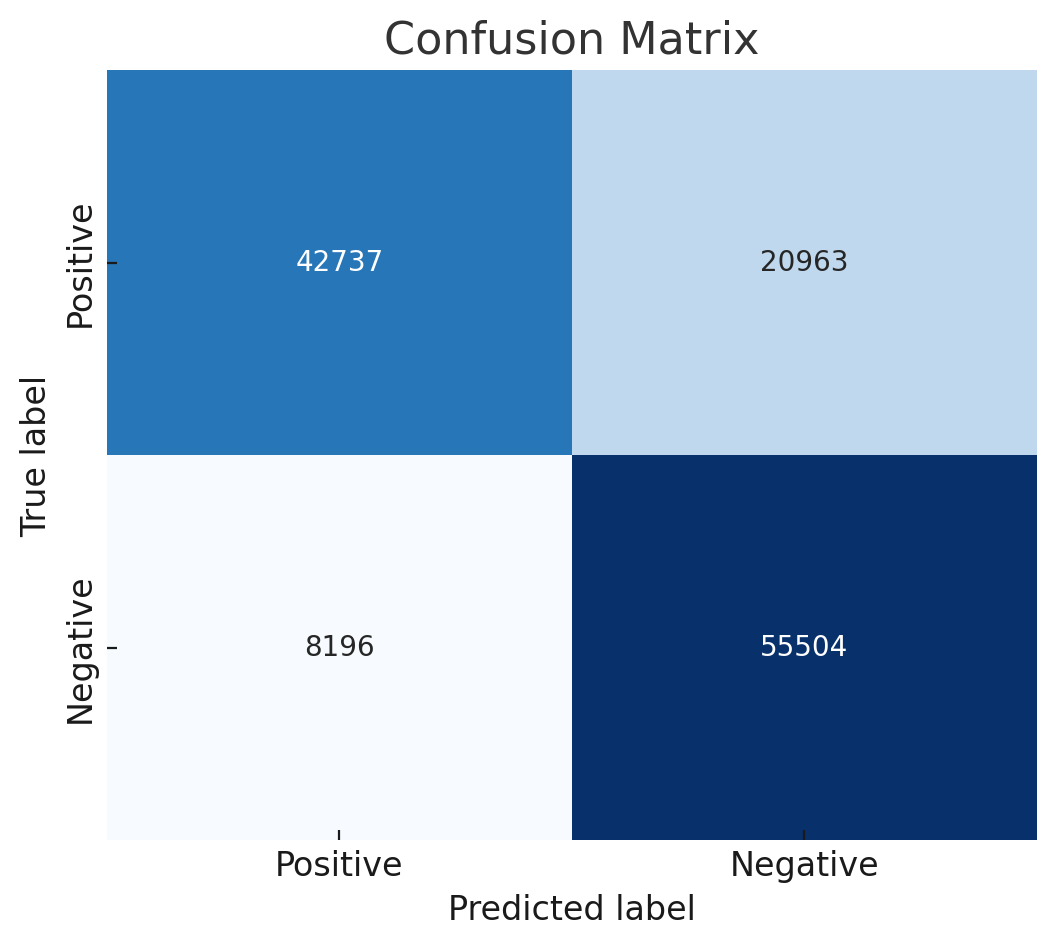
\includegraphics[width=0.6\textwidth]{ressources/xfeat_cm.png}
    \caption{Evaluation results comparison}
    \label{fig:evaluation_results}
\end{figure}
\begin{table}[H]
    \centering
    \renewcommand{\arraystretch}{1.2}
    \begin{tabular}{lcccc}
        \toprule
        \textbf{Class}        & \textbf{Precision} & \textbf{Recall} & \textbf{F1-score} & \textbf{Support} \\
        \midrule
        No Match              & 0.73               & 0.87            & 0.79              & 63,700           \\
        Match                 & 0.84               & 0.67            & 0.75              & 63,700           \\
        \midrule
        \textbf{Accuracy}     &                    &                 & 0.77              & 127,400          \\
        \textbf{Macro Avg}    & 0.78               & 0.77            & 0.77              & 127,400          \\
        \textbf{Weighted Avg} & 0.78               & 0.77            & 0.77              & 127,400          \\
        \bottomrule
    \end{tabular}
    \caption{Classification report on XFeat.}
    \label{tab:classification_report}
\end{table}
Compared to our models' performance:
\begin{table}[H]
    \centering
    \renewcommand{\arraystretch}{1.2}
    \begin{tabular}{lcccc}
        \toprule
        \textbf{Class}        & \textbf{Precision} & \textbf{Recall} & \textbf{F1-score} & \textbf{Support} \\
        \midrule
        No Match              & 0.79               & 0.84            & 0.81              & 63,700           \\
        Match                 & 0.83               & 0.77            & 0.80              & 63,700           \\
        \midrule
        \textbf{Accuracy}     &                    &                 & 0.81              & 127,400          \\
        \textbf{Macro Avg}    & 0.81               & 0.81            & 0.81              & 127,400          \\
        \textbf{Weighted Avg} & 0.81               & 0.81            & 0.81              & 127,400          \\
        \bottomrule
    \end{tabular}
    \caption{Classification report with precision, recall, F1-score, and support for the two classes.}
    \label{tab:classification_report2}
\end{table}
Overall, the model achieved an accuracy of \textbf{75\%}. However, it performed better at identifying ``No Match'' pairs than at detecting all the ``Match'' pairs. The model is very cautious about calling something a ``Match''. When it does, it is usually correct, but it misses many true matches.

\subsubsection*{Detailed Breakdown}

Here is what each term means in the context of the results:

\begin{itemize}
    \item \textbf{Precision:} Of all the times the model predicted a certain class, how often was it correct?
          \begin{itemize}
              \item \textbf{No Match (0.79):} When the model predicted ``No Match'', it was correct only 79\% of the time.
              \item \textbf{Match (0.83):} When the model predicted ``Match'', it was correct 83\% of the time. This is high and means the model produces fewer false positives.
          \end{itemize}

    \item \textbf{Recall:} Of all the actual instances of a class, how many did the model correctly identify?
          \begin{itemize}
              \item \textbf{No Match (0.84):} The model correctly identified 84\% of all actual ``No Match'' pairs.
              \item \textbf{Match (0.77):} The model only found 77\% of all the true ``Match'' pairs. This means it missed 23\% of them, leading to many false negatives.
          \end{itemize}

    \item \textbf{F1-Score:} The harmonic mean of Precision and Recall. It balances the trade-off between the two. The model has a decent F1-score for both classes, but the lower recall for ``Match'' reduces its value.

    \item \textbf{Support:} The number of actual occurrences of each class in the dataset.
\end{itemize}

\subsubsection*{Averages}

\begin{itemize}
    \item \textbf{Accuracy (0.81):} The overall percentage of correct predictions (81\% of 63,700 pairs).
    \item \textbf{Macro Avg (0.81, 0.81, 0.81):} The unweighted average across both classes, treating ``Match'' and ``No Match'' equally.
    \item \textbf{Weighted Avg (0.81, 0.81, 0.81):} The average weighted by the number of samples. Since there are more ``Match'' pairs, the average is biased towards their scores.
\end{itemize}

\subsubsection*{In Simple Terms}

The model is very conservative, it avoids calling something a match unless it
is very certain.

\begin{itemize}
    \item \textbf{Good news:} When it says ``Match'', we can trust it (81\% precision).
    \item \textbf{Bad news:} It fails to identify a quarter of the actual matches (77\% recall), classifying them instead as ``No Match''.
\end{itemize}
\subsection{Trade-offs: Speed vs. Accuracy}
\begin{tabular}{l r r r r r r r r}
\toprule
Method    & Extraction(s) & Speedup & Matching(s) & Speedup & Total(s) & Speedup & Matches & Matches/s \\
\midrule
SIFT-CPU  & 0.1420 & 1.0  & 0.0024 & 0.63 & 0.1443 & 1.0  & 579  & 244319 \\
XFeat-GPU & 0.0117 & 12.1 & 0.0015 & 1.0  & 0.0132 & 10.9 & 256  & 19394  \\
XFeat-CPU & 0.0110 & 12.9 & 0.0006 & 2.5  & 0.0116 & 12.4 & 256  & 220690 \\
\bottomrule
\end{tabular}


\vspace{1em}

The results highlight a pronounced contrast between SIFT and XFeat in terms of computational efficiency. 
XFeat demonstrates a substantial speed advantage, outperforming SIFT across extraction, matching, and total runtime.
Notably, XFeat achieves these gains even on the CPU, underscoring its efficiency and making it a strong candidate 
for deployment in environments where GPU resources are limited or unavailable. 
However, this gain in speed comes at the cost of accuracy. While XFeat delivers results an order of magnitude faster, 
its number of matches is significantly lower than SIFT's, which translates into reduced reliability in many 
feature-matching tasks. SIFT, despite being slower, provides at least 15\% higher accuracy, which can be 
critical in applications where precision is more important than raw throughput. 
Overall, these findings illustrate the fundamental trade-off between speed and accuracy: XFeat offers 
exceptional performance efficiency, while SIFT remains more robust in terms of match quality.

\subsection{Visual Results on Gaming Footage}

\section{Computational Efficiency}
\subsection{FPS and Latency Benchmarks}
\subsection{Memory and CPU Usage Profiles}
